% !TEX root = ./main.tex

\section{Determining and removing an equilibration or `burn-in' portion of a trajectory}
\label{sec:equil}

\begin{figure}
  \centering
  % 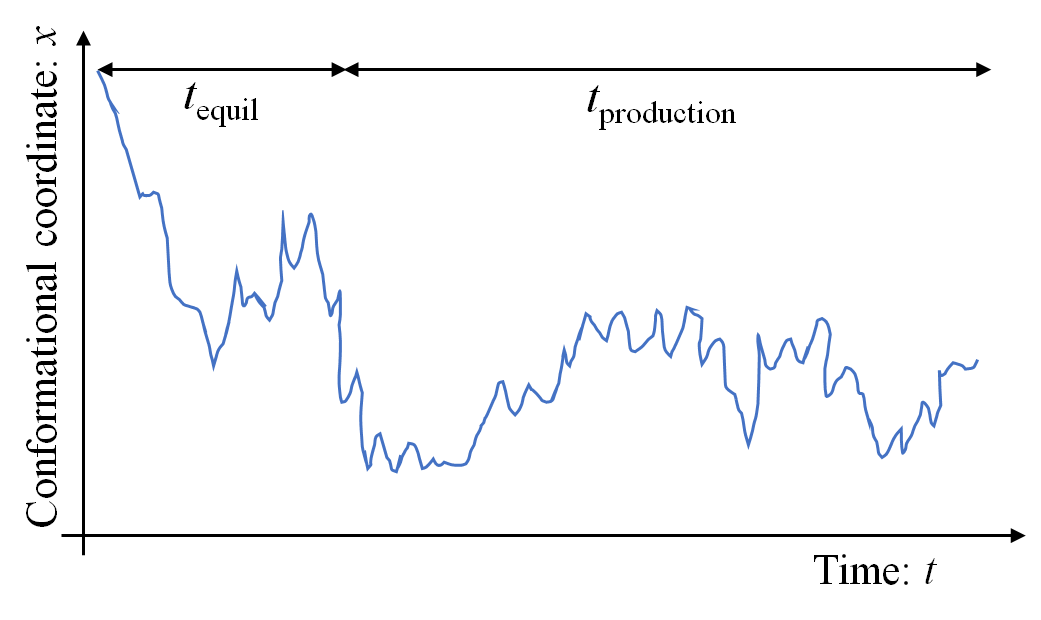
\includegraphics[width=7cm]{figures/tequil-time-trace}
  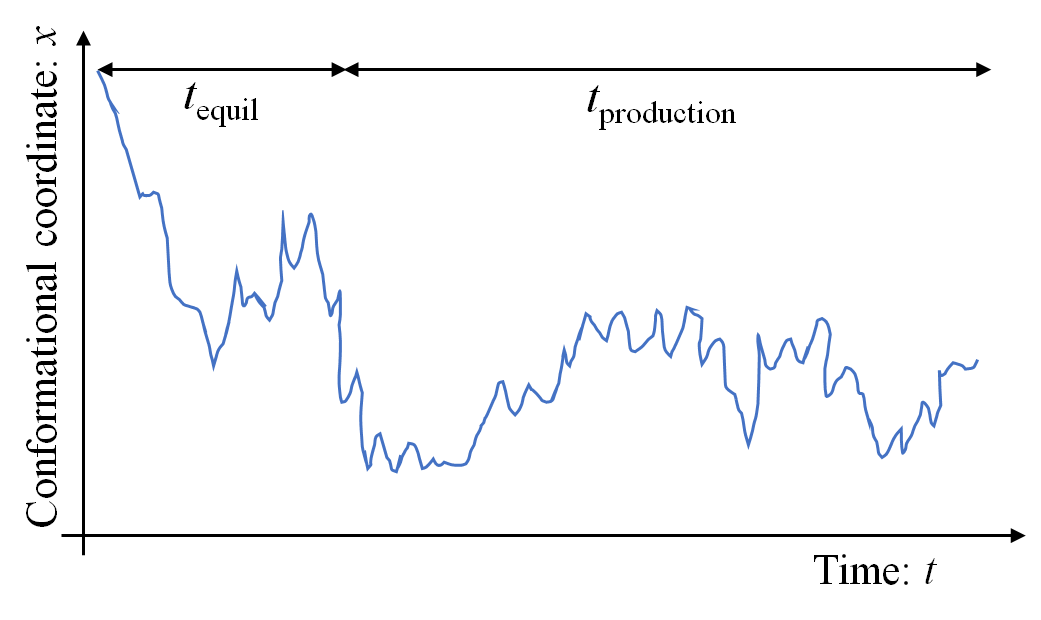
\includegraphics[width=0.9\linewidth]{figures/tequil-time-trace}
  \caption{
  \label{fig:tequil}
  The equilibration and production segments of a trajectory.
  ``Equilibration'' over the time $t_{\mathrm{equil}}$ represents transient behavior while the initial configuration relaxes toward configurations more representative of the equilibrium ensemble.
  Readers are encouraged to select $t_{\mathrm{equil}}$ in a systematic way based on published literature.
  If you find strong sensitivity of ``production'' data to the choice of $t_{\mathrm{equil}}$, this suggests additional sampling is required.
  }
\end{figure}

The ``equilibration'' or ``burn-in'' time $t_{\mathrm{equil}}$ represents the initial part of a single continuous trajectory (whether from MD or MC) that is \emph{discarded} for purposes of data analysis of \emph{equilibrium properties};
the remaining trajectory data is often called ``production'' data.
See Fig.\ \ref{fig:tequil}.
Discarding data may seem counter-productive, but there is no reason to expect that the initial configurations of a trajectory will be important in the ensemble ultimately obtained.
Including early-time data, therefore, can systematically \emph{bias} results.

%\textcolor{red}{PNP Comment: I rephrased the next two paragraphs consistent with my understanding of what they were trying to say. Original text is commented out in latex.  Please verify what I have written is representative of what was intended.}

To illustrate these points, consider the process of relaxing an initial, crystalline configuration of a protein to its amorphous counterpart in an aqueous environment.
While the initial structure might seem to be intrinsically valuable, remember that configurations representative of the crystal structure may never appear in an aqueous system.
%Perhaps worse, the force field used for aqueous interactions will in general be different from its crystalline counterpart, so that we cannot realistically hope to even model the latter.  \textcolor{green}{DMZ: The preceding is not generally true for biomolecules so we should omit the sentence or revise accordingly.} \textcolor{blue}{DWS: Agree with DMZ, this sentence is not generally true.}
As a result, the initial structure may be subject to unphysical forces and/or transitions that provide useless, if not misleading information about the system behavior.\footnote{In MD modeling of structural polymers (e.g.\ thermoset polymers), the problem of unphysical forces can be so severe that simulations become numerically unstable and crash.  This frequently manifests as systems that explode and/or tear themselves apart.  As a result, relaxation is often performed using Monte Carlo moves that minimize energy without reference to velocities and forces.}
Relaxation should therefore be viewed as a means to an end: we only care that the relaxed state is representative of {\it any} local energy-minimum that the system might sample, not how we arrived at that state.
%\textcolor{green}{DMZ: I changed 'final state' to 'relaxed state' because I didn't want to suggest that relaxation is the final goal of simulation.}

The RMSD trace in Fig. \ref{f:rmsd} illustrates typical behavior of a system undergoing relaxation.  Note the very rapid RMSD increase in the first $\sim$200 ns. Part of this increase is simply entropic: the volume of phase space within 1 {\AA} of a protein structure is extremely small, so that the process of thermalizing rapidly increases the RMSD from the starting structure, \emph{regardless of how favorable or representative that structure is}.  Thus, examining that initial rapid increase is not helpful in determining an equilibration time.  However, in this case, the RMSD continues to increase past 3 {\AA}, which is larger than the amplitude of simple thermal fluctuations (shown by Fig.\ \ref{f:rmsd}B), indicating an initial drift to a new structure, followed by sampling.

%In the biomolecular realm, consider the initial configuration of a protein, which has been energy-minimized and otherwise relaxed from a crystal structure.  %PNP comment: lightly edited these few sentences
%While such an initial structure might seem to be intrinsically valuable, remember that configurations important in a crystal environment may not be equally pertinent to an aqueous environment due to e.g. crystal packing etc. 
%Also, any energy minimization/relaxation that has been performed likely will be very local and keep the configuration within or nearby the initial energy basin.  Moreover, the force field used to represent interactions will in general not be identical to that used to as part of the crystal structure solution.  See the RMSD trace in Fig.\ \ref{f:rmsd}, and note the very rapid RMSD increase in the first $\sim$200 ns. Part of this increase is simply entropic: the volume of phase space within 1 {\AA} of a protein structure is extremely small, so the process of thermalizing rapidly increases RMSD from the starting structure, \emph{regardless of how favorable or representative that structure is}.  Thus, examining that initial rapid increase is not helpful in determining an equilibration time.  However, in this case, the RMSD continues to increase past 3 {\AA}, which is larger than the amplitude of simple thermal fluctuations (shown by Fig.\ \ref{f:rmsd}B), indicating an initial drift to a new structure, followed by sampling.

%PNP comment: not sure what the next paragraph has to offer.  I commented it out.
%In materials science, if a simulation is designed to study thermally induced fluctuations or defects in a (mostly) ordered system,
%an initial fully ordered configuration is not likely to be representative of the targeted ensemble, and the early dynamics represent a transient relaxation toward the average, which is not representative of the desired equilibrium ensemble.

Accepting that some data should be discarded, it is not hard to see that we want to avoid discarding too much data, given that many systems of interest are extremely expensive to simulate.  In statistical terms, we want to remove bias but also minimize uncertainty (variance) through adequate sampling.  Before addressing this problem, however, we emphasize that the very notion of separating a trajectory into equilibration and production segments only makes sense if the system has indeed reached configurations important in the equilibrium ensemble. While it is generally impossible to guarantee this has occurred, some easy checks for determining that this has not occurred are described in Sec.\ \ref{sec:quick}. \emph{It is essential to perform those basic checks before analyzing data with a more sophisticated approach} that may assume a trajectory has a substantial amount of true equilibrium sampling.

%\textcolor{red}{PNP comment: The below paragraph has a few ambiguities. See .tex file for my comments}
%\textcolor{green}{DMZ comment: I made some edits but it's not really my expertise.  I will ask John Chodera to clean it up for us.}
%PNP comment:  The sentence, "The key idea is to analyze data as a function of the amount of data removed," sounds oxymoronic.  Is the idea to track estimators of an observable as data in the corresponding time-series is removed?  If so, consider rephrasing.  Also, how is bias monitored if we don't know the true value of the observable?  This needs to be flushed out a little more.  Also, how can the effective sample size increase as I remove data...?  I suspect that the burn-in time shifts the mean if I keep all of the data, so I have the appearance of small but long-time correlations.  If this intuition is correct, we should probably be a little more explicit.

A robust approach to determining the equilibration time is discussed in \cite{Chodera-2016}, which generalizes the notion of reverse cumulative averaging~\cite{Yang2004} to observables that do not necessarily have Gaussian distributions.
%The key idea is to analyze data iteratively as an increasing amount of the time series is removed - i.e., as $t_{\mathrm{equil}}$ increases from zero.  
The key idea is to analyze timeseries data considering the effect of discarding various trial values of the initial equilibration interval, $t_{\mathrm{equil}}$ (Fig.\ \ref{fig:tequil}), and selecting the value that maximizes the effective number of uncorrelated samples of the remaining production region.
This effective sample size is estimated from the number of samples in the production region divided by the number of temporally correlated samples required to produce one effectively uncorrelated sample, based on an auto-correlation analysis.
At sufficiently large $t_{\mathrm{equil}}$, the majority of the initial relaxation transient is excluded, and the method selects the largest production region for which correlation times remain short to maximize the number of uncorrelated samples.
Care must be taken in the case that the simulation is insufficiently long to sample many transitions among kinetically metastable states, however, or else this approach can simply result in restricting the production region to the last sampled metastable basin.
%As described by Chodera \cite{Chodera-2016}, one can monitor both the variance and the effective sample size, which is roughly quantified by the total simulation time considered divided by the auto-correlation time.
%If the transient data in the interval $t_{\mathrm{equil}}$ is anomalous and removed, one expects the variance to decrease.
%Chodera indicates that the effective sample size peaks at the optimal $t_{\mathrm{equil}}$, making the latter easy to discern.
%We caution that estimating the correlation time may require care, and 
Readers may want to compare auto-correlation times for individual observables to the global 'decorrelation time' \cite{Lyman2007a} described in Sec.\ \ref{sec:global}.  
As another general check, if values of observables estimated from the production phase depend sensitively on the choice of $t_{\mathrm{equil}}$, it is likely that further sampling is required.


